\documentclass[12pt]{article}

\usepackage{graphicx}
\usepackage{paralist}
\usepackage{amsfonts}
\usepackage{amsmath}
\usepackage{hhline}
\usepackage{booktabs}
\usepackage{multirow}
\usepackage{multicol}
\usepackage{url}
\usepackage{hyperref}

\oddsidemargin -10mm
\evensidemargin -10mm
\textwidth 160mm
\textheight 200mm
\renewcommand\baselinestretch{1.0}

\pagestyle {plain}
\pagenumbering{arabic}

\newcounter{stepnum}

%% Comments

\usepackage{color}

\newif\ifcomments\commentstrue

\ifcomments
\newcommand{\authornote}[3]{\textcolor{#1}{[#3 ---#2]}}
\newcommand{\todo}[1]{\textcolor{red}{[TODO: #1]}}
\else
\newcommand{\authornote}[3]{}
\newcommand{\todo}[1]{}
\fi

\newcommand{\wss}[1]{\authornote{blue}{SS}{#1}}

\title{Assignment 4, Design Specification}
\author{SFWRENG 2AA4}

\begin {document}

\maketitle
This Module Interface Specification (MIS) document contains modules, types and
methods used to support the popular game 2048. At the start of the game, the player
will be provided with a sixteen tile game board where there will be two tiles 
occupied at a random position within the game board with the number 2. The goal
of the game is to merge tiles with the same number as many times as possible in
order to reach a tile numbered 2048. The player will be able to merge tiles through
using the usage of the controller. The controller will allow for the player to move
left, right, up, down. Each time the player uses the controller to make move left,
right, up, down; the game will spawn a new numbered tile which is either numbered 2
or 4 at any position within the game board. Each player will start with a score of 0.
Each time two tiles are combined together, the mathematical sum of the two tiles
will be added to the score of the player.

  \begin{center}
  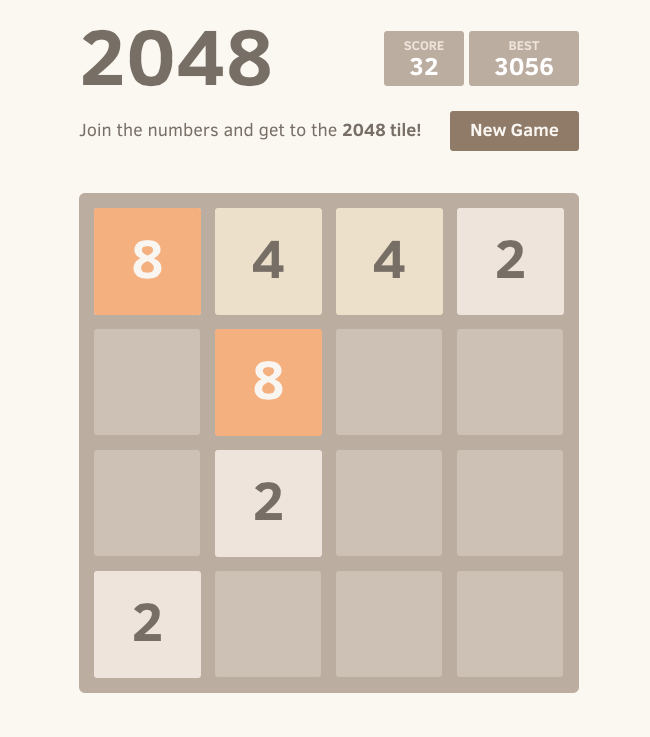
\includegraphics[scale = 0.3]{sampleboard2}
  
  The above board visualization is from https://www.omgubuntu.co.uk/2014/03/install-2048-on-ubuntu-download
  \end{center}

\newpage

\section{Overview of the design}

This design has three modules which are able to maintain the state of the game as well as the view of the game board. The $Board.java$ module is used to 
store information about the game, get the score,the grid as well as the control. The $Direction.java$ module is a module which stores information regarding 
the way the user can prompt movement on the game board as well get the x and y components of the grid. These movements include $up,down,left,right$ by the 
user.

\subsection*{Likely Changes my design considers:}

\begin{itemize}
  \item Changing the way the tiles look within the game board as the value of the tile increases
  \item The way every move the players makes within the game is stored
  \item Changing minor details regarding how a new tile is spawned
  \item Making sure the consistency of the way the tiles are spawned or the way the tiles are merged together 
        regardless of whether the player finishes the game or not.
\end{itemize}

\newpage

\section* {Board Module}

\subsection*{Template Module}

Board

\subsection* {Uses}

None

\subsection* {Syntax}

\subsubsection* {Exported Constants}

None

\subsubsection* {Exported Types}

Board = ?

\subsection* {Semantics}

\subsubsection* {State Variables}

$\mathit{NUMSTARTTILES}: \mathbb{N}$\\
$TWOPROBABILITY: \mathbb{N}$\\
$GRIDSIZE: \mathbb{N}$\\
$RANGE: \mathbb{N}$\\
$TILETWO: \mathbb{N}$\\
$TILEFOUR: \mathbb{N}$

\subsubsection* {State Invariant}

None

\subsubsection* {Assumptions}

None

\newpage

\section* {Direction Module}

\subsection*{Module}

Direction

\subsection* {Uses}

None

\subsection* {Syntax}

\subsubsection* {Exported Constants}

None

\subsubsection* {Exported Types}

None

\subsection* {Semantics}

\subsubsection* {State Variables}

$\mathit{y}$: $\mathbb{N}$\\
$\mathit{x}$: $\mathbb{N}$

\subsubsection* {State Invariant}

None

\subsubsection* {Assumptions}

None

\section*{Critique of Design}

\begin{itemize}
  \item The design is very consistent in terms of the usage of the language and terminology being used in each module. Within each specification, the names
        of state variables or methods do not change at all. The advantage of having a consistent specification is that a person reading the specification for
        the first time will be able to understand how the module is being constructed without any confusion. The specifications have no homonyms or synonyms
        which prevents any further issues. In addition to the same naming conventions, the order of which each program is accessed maintains a level of
        consistency.
  \item The design maintains a level of essentiality as well because it does not have any unnecessary programs. Whatever is specified within the design
        specification is what exists within the modules implemented for the state of the game and the view of the gameboard.
  \item The design maintains generality resulting in no one module being limited to one particular case and tend to work together to allow for the user to
        have the best experience while playing the game. All modules (unless specifically limited due to the rules of the game) are free from any restriction
        or limitation and allows for each module to have a long lifespan.
  \item 
\end{itemize}

\section*{Answers to Questions:}

Q1: Draw a UML diagram for the modules in A3.

\begin{center}
  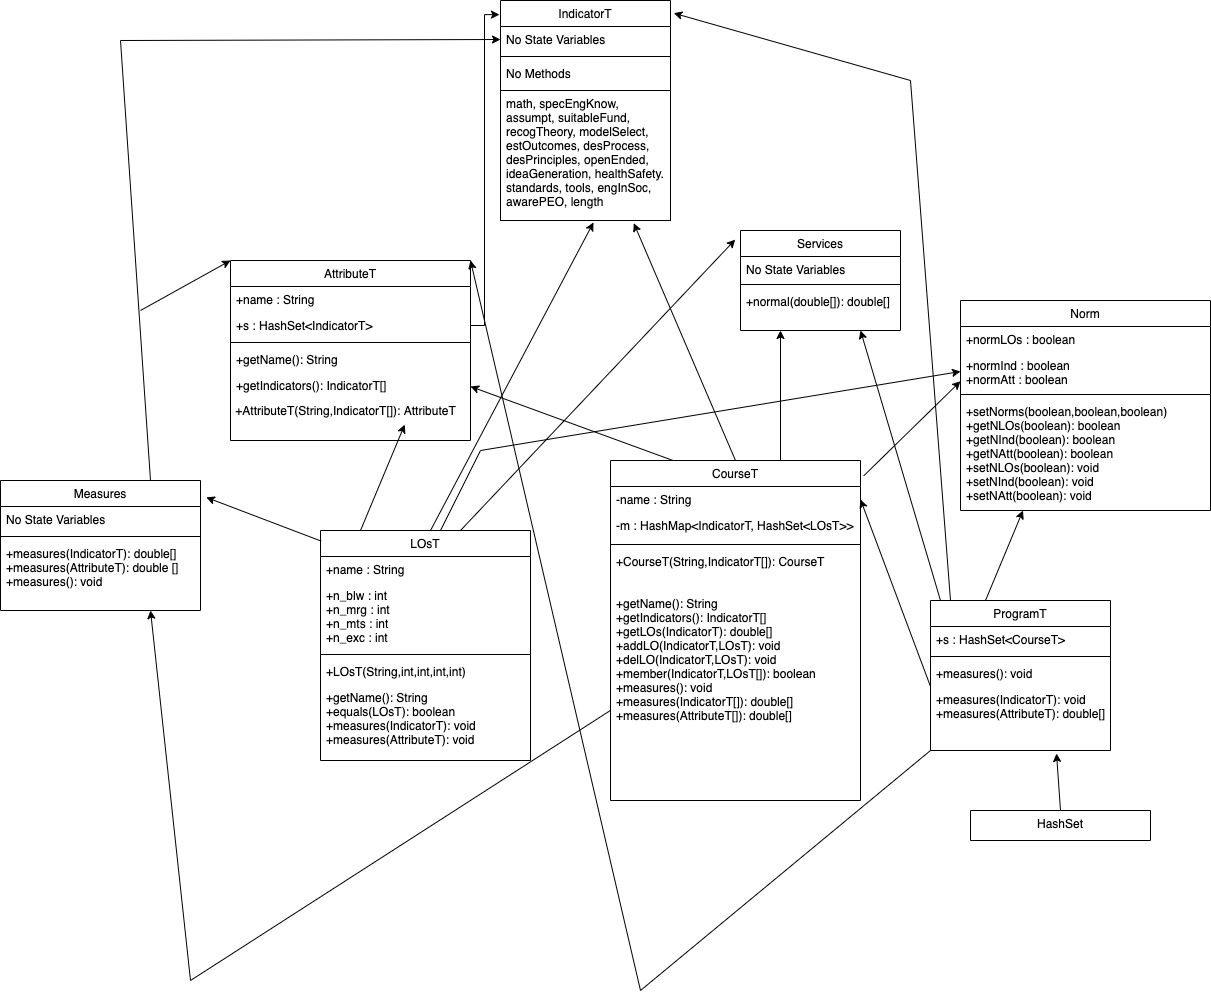
\includegraphics[scale = 0.3]{A3UMLsemi.png} \\
  The UML is constructed using https://app.diagrams.net/
\end{center}


\noindent Q2: Draw a control flow graph for the convex hull algorithm.  The graph should
  follow the approach used by the Ghezzi et al.\ textbook.  In particular, the
  code statements should be edges of the graph, not nodes.  Code for the convex
  hull algorithm can be found at:
  \href{https://startupnextdoor.com/computing-convex-hull-in-python/}
  {https://startupnextdoor.com/computing-convex-hull-in-python/}.  To match the
  diagrams available from Ghezzi, replace the for loop in the code with a while
  loop.


\begin{center}
  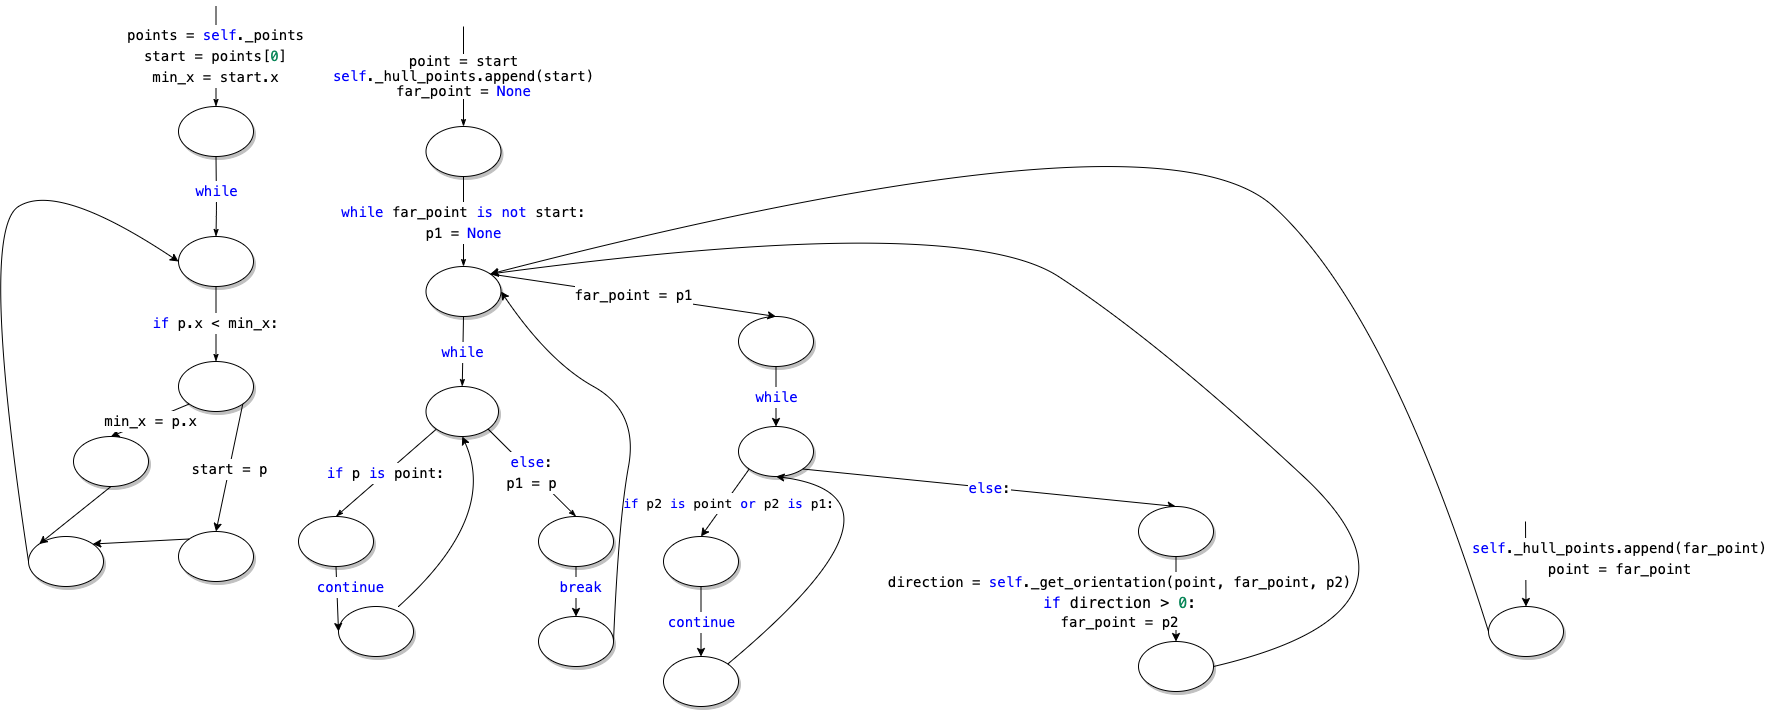
\includegraphics[scale = 0.3]{ConvexHullsemis.png} \\
  The control flow graph is constructed using https://app.diagrams.net/
\end{center}

\end {document}
